\documentclass[11pt,a4paper]{article}
\usepackage[margin=1in]{geometry}
\usepackage[T1]{fontenc}
\usepackage[utf8]{inputenc}
\usepackage{lmodern,microtype}
\usepackage{amsmath,amssymb,amsthm,mathtools}
\usepackage{graphicx,booktabs,tabularx,array,multirow}
\usepackage{float,caption,subcaption}
\usepackage{algorithm,algpseudocode}
\usepackage{tikz}
\usetikzlibrary{arrows.meta,positioning,fit,calc,shapes.geometric}
\usepackage[backend=biber,style=numeric,sorting=none]{biblatex}
\addbibresource{references.bib}
\usepackage[hidelinks,hypertexnames=false]{hyperref}
\usepackage{cleveref}
\usepackage{enumitem}
\usepackage{url}
\setlength{\emergencystretch}{3em}
\captionsetup{font=small,labelfont=bf}
\newtheorem{proposition}{Proposition}
\newtheorem{lemma}{Lemma}
\newcommand{\Opt}{\operatorname{Opt}}
\newcommand{\Goal}{\operatorname{Goal}}
\newcommand{\Valid}{\operatorname{Valid}}
\newcommand{\Cost}{\operatorname{Cost}}
\title{The Geometry of Natality: Creation-Enabled Reachability and Cost-Optimal Repair in Dependency Graphs}
\author{Mohammad Amir Khusru Akhtar\\\small Usha Martin University, Ranchi, Jharkhand, India}
\date{}
\begin{document}
\maketitle
\begin{abstract}
Repair in a dependency network may require more than restoring an existing vertex: a replacement must be introduced, made operational, and connected to the services that depend on it. We study this distinction through a creation-enabled, costed transition system for evolving dependency graphs. Its states retain component identity, operational status, dependencies, and action history; admissible transitions include restoration, creation, and rewiring. A directed extended path-cost function makes the reachability and optimization questions precise without presuming metric symmetry. We establish elementary but informative separation and cost-comparison statements for creation-enabled versus restoration-only planning, and state the assumptions under which independent repair subproblems decompose exactly. A three-service instance admits two minimum-cost strategies of cost three. Across 12 synthetic search instances, exhaustive enumeration and uniform-cost search agree on the optimum; for four independent groups, enumeration visits 314,217 search nodes and uniform-cost search expands 399 states. A further 24 synthetic cases exercise guarded decomposition, including a shared-capacity counterexample to unqualified plan composition. We also formalize fresh-name equivalence and prove cost preservation for equivariant identity quotients, while separating a small executable symmetry check from unperformed comparative experiments. These findings provide an explicit formal vocabulary and reproducible correctness evidence for creation-aware recovery; they do not establish a new graph-transformation calculus or superiority over established planning and verification tools.
\end{abstract}
\noindent\textbf{Keywords:} dependency graph; graph transformation; cost-optimal repair; service recovery; component creation; state-space search; decomposition

\section{Introduction}
Repairing a failed dependency is not always a matter of bringing the failed component back. A replacement may be created, yet the system remains unavailable until its dependents are redirected. The cost of recovery therefore belongs not to an isolated repair operation but to a sequence of changes in a graph. This distinction motivates the \emph{geometry of natality}: a view of repair in which the creation of components is represented explicitly, alongside the relationships that make the new components operational.

Graph transformation provides established machinery for changing and analyzing structured states \cite{Ehrig2006,Konig2018}; GROOVE makes this machinery executable for state-space exploration \cite{Rensink2004,Ghamarian2012}. Abstraction, state-space reduction, and graph-based verification have long histories \cite{Burch1992,Emerson2005,Rensink2004Comparison,Konig2025}. Consequently, creation-aware graph planning cannot be treated as novel merely because its states contain newly created vertices. The question addressed here is more specific: what can be established, by exact search and independent checks, about cost-optimal repair when a failed component can be restored or replaced?

We make three contributions. First, we define a finite repair-planning model that keeps graph structure, action history, and recovery conditions explicit. Second, we construct a small auditable recovery instance and a parameterized family in which two independent exact procedures agree on minimum cost. Third, we identify a precise decomposition boundary: independent local repairs compose optimally, whereas shared restrictions can invalidate locally selected plans. The analysis separates what follows from the availability of creation actions from what follows solely from standard shortest-path and decomposition principles.

\section{Background and relation to established methods}
Dependency graphs are a natural representation of systems in which the availability of one component depends on another; graph structure and network function need not coincide \cite{Newman2003}. Graph-rewriting rules can represent changes to both nodes and edges \cite{Ehrig2006,Konig2018,Plump1999}. The distinguishing modelling decision in this work is to expose replacement creation and subsequent rewiring as separate, costed actions rather than collapse them into a single abstract recovery event.

The choice has consequences for search. Two configurations with the same number of live components may differ in which dependency is satisfied. Furthermore, two states with the same graph may admit different future actions when rules have history-dependent prerequisites. For exact exploration, the state key must therefore retain all information that affects future applicability and the recovery predicate. The comparison in \Cref{tab:prior} situates the present work without asserting superiority over existing tools.

\begin{table}[H]\centering\caption{Scope of the present formulation relative to established approaches.}\label{tab:prior}\small
\begin{tabularx}{\linewidth}{@{}p{0.26\linewidth}X X@{}}\toprule
Approach & Established capability & Relationship to this study\\\midrule
Graph transformation \cite{Ehrig2006,Konig2018} & Rule-based changes to graph structure & Provides the underlying conceptual vocabulary\\
GROOVE \cite{Ghamarian2012} & Executable exploration of graph-transformation systems & Relevant future matched implementation; no matched results claimed\\
State-space reduction \cite{Emerson2005,Konig2025} & Reduction and abstraction of verification spaces & Prevents attributing generic reduction ideas to natality\\
Present exact search & Explicit costs, action prerequisites, replacement creation, and recovery goals & Verified on synthetic instances; no new search complexity guarantee\\\bottomrule
\end{tabularx}\end{table}

\subsection{Related structural and optimization perspectives}
Classical depth-first graph algorithms clarify the role of connectivity and structural decomposition in dependency analysis \cite{Tarjan1972}; network topology alone does not specify recovery feasibility \cite{Newman2003}. The distinction between graph structure and an operational objective also appears in influence maximization \cite{Kempe2003} and submodular optimization \cite{Nemhauser1978}, although neither directly solves the action-sequencing problem considered here. Graph augmentation \cite{Eswaran1976} changes connectivity, whereas precedence-constrained optimization formalizes choices subject to dependency restrictions \cite{Boyd1993,You2007,Espinoza2015}. These are adjacent problems, not substitutes for a stateful repair planner.

Name generation in nominal rewriting \cite{Fernandez2005} and graph passing \cite{GhamarianGraphPassing2012} provide formal context for newly introduced graph objects. Confluence analysis \cite{Campbell2021} concerns the relationships among rewriting paths; model-transformation validation \cite{Adam2026} and learning-based graph-transformation testing \cite{Ghasemi2026} investigate different verification strategies. GROOVE has also supported reaction-system experiments \cite{Bruni2025}. These studies motivate separating representational adequacy, optimality of the search procedure, and empirical comparison of tools. They do not establish a performance advantage for the present implementation.

\section{Creation-enabled state space and operational geometry}
A repair system is described by a tuple
\begin{equation}\label{eq:gonspace}
\mathcal{N}=(\mathcal{S},\mathcal{A},T,c,\Gamma,\Phi),
\end{equation}
where $\mathcal{S}$ is a set of identity-bearing attributed dependency graphs with action histories, $\mathcal{A}$ is a set of typed actions, $T$ is a partial transition map, $c:\mathcal{A}\to\mathbb{R}_{\geq0}$ assigns costs, $\Gamma\subseteq\mathcal{S}$ identifies admissible states, and $\Phi\subseteq\Gamma$ is the recovery goal. The general model may have infinitely many states when creation draws fresh identities from an unbounded supply. The exact-search claims below apply only to finite instances with a fixed finite action alphabet, bounded fresh identities, and single-use actions; the experiments satisfy these restrictions. The identity of a newly created component is distinct from the identity of the failed component even when both implement the same service role. This matters because dependencies refer to particular vertices, not merely to service labels.

We distinguish three kinds of transition. A \emph{restoration} changes the operational attributes of an existing vertex without introducing a new identity. A \emph{creation} introduces a fresh vertex identity into the graph; the newly created component need not yet serve any dependent. A \emph{rewiring} changes dependency edges without introducing a new vertex. These types are modelling distinctions, not claims that existing graph-rewriting formalisms lack the ability to represent them \cite{Ehrig2006,Konig2018,Fernandez2005}.

Let $\mathcal{A}_{0}$ contain all admissible creation-free actions, including restoration and rewiring, and let $\mathcal{A}_{+}$ additionally permit creation. Thus the restricted model is creation-free, not necessarily restoration-only. For a fixed initial state $s$, write $\mathcal{R}_{0}(s)$ and $\mathcal{R}_{+}(s)$ for the states reachable by valid finite paths under the respective action sets. A directed extended operational distance is
\begin{equation}\label{eq:distance}
d_{+}(s,t)=\inf_{\substack{\pi:s\leadsto t\\\pi\ \mathrm{admissible}}}\ \sum_{a\in\pi}c(a),\qquad \inf\varnothing=+\infty.
\end{equation}
The same definition with paths restricted to $\mathcal{A}_{0}$ gives $d_{0}$. Concatenation of admissible paths yields the directed triangle inequality whenever the relevant paths exist. In general $d_{+}(s,t)\ne d_{+}(t,s)$, and distinct states may be connected at zero cost; this construction is therefore not asserted to be a metric. Its value lies in making operational reachability and cost explicit rather than assigning an unsupported geometric interpretation to graph drawings.

\begin{proposition}[Reachability and cost monotonicity under added actions]\label{prop:monotone}
Assume the two models have identical initial states, common-action transitions, costs, admissibility constraints, and goals, and differ only because $\mathcal{A}_{0}\subseteq\mathcal{A}_{+}$. Then $\mathcal{R}_{0}(s)\subseteq\mathcal{R}_{+}(s)$, and the optimal goal-reaching costs satisfy $\Opt_{+}(s)\leq\Opt_{0}(s)$, with $+\infty$ allowed.
\end{proposition}
\begin{proof}
Every path using only $\mathcal{A}_{0}$ is also an admissible path in the expanded system, by the common-transition and common-constraint assumptions. Reachable-state inclusion follows. Taking the infimum over a superset of feasible goal-reaching paths cannot increase its value.
\end{proof}

The inequality can be strict, but need not be. For example, if restoration costs five units and creation followed by rewiring costs three, with both routes reaching the same recovery goal, then $\Opt_{+}=3<5=\Opt_{0}$. This is a constructed example illustrating the proposition, not a measured result. In the evaluated fixture, both routes cost three, so creation does not strictly improve the optimum.

\begin{proposition}[Creation-essential recovery]\label{prop:essential}
Under the assumptions of \Cref{prop:monotone}, creation is necessary for reaching a goal from $s$ exactly when $\mathcal{R}_{0}(s)\cap\Phi=\varnothing$ and $\mathcal{R}_{+}(s)\cap\Phi\ne\varnothing$.
\end{proposition}
\begin{proof}
The first condition states that no creation-free admissible path reaches a goal; the second exhibits a goal-reaching path in the expanded system. Conversely, if a goal is reachable only through a path that uses creation, it cannot belong to $\mathcal{R}_{0}(s)$ but belongs to $\mathcal{R}_{+}(s)$.
\end{proof}

For a concrete separation, consider a failed service whose restoration action is forbidden by policy, while creation of a replacement and redirection of its dependent are permitted. The creation-free goal set is unreachable; the creation-enabled system reaches the goal after the two permitted operations. This small construction isolates a difference in \emph{feasible action sets}, not a representational impossibility for established graph-transformation systems. The propositions are direct consequences of transition-system inclusion, and no novelty is claimed for the underlying mathematical principle.

\begin{table}[H]\centering\caption{Operational distinctions in the creation-enabled model.}\label{tab:foundations}\small
\begin{tabularx}{\linewidth}{@{}p{0.23\linewidth}XX@{}}\toprule
Operation & Identity and structure & Recovery implication\\\midrule
Restoration & Preserves vertex identity; changes attributes & Can restore existing dependencies\\
Creation & Adds a fresh vertex identity & Does not itself redirect dependents\\
Rewiring & Preserves vertex set; changes edges & Can connect dependents to a replacement\\
Combined plan & May change identities, attributes, and edges & Must satisfy the same goal and constraints\\\bottomrule
\end{tabularx}\end{table}
The distinction between these operations is summarized in \Cref{tab:foundations}. It permits explicit tests of whether the ability to create components changes feasible recovery paths or their minimum cost.

\section{Finite repair states, actions, and objectives}
Let a dependency graph be $G=(V,E,\ell)$, where $(u,v)\in E$ means that component $u$ depends on component $v$, and $\ell(v)$ records whether $v$ is operational. A repair state is $s=(G,H)$, where $H\subseteq A$ records actions already performed. In the evaluated single-use rules, the set $H$ is sufficient: prerequisites test whether a named action has occurred, not the order of multiple prior actions. For genuinely order-sensitive policies, the state must instead retain an appropriate ordered history or sufficient automaton state. A finite action $a\in A$ has a partial transition $T_a$, an applicability predicate $P_a$, and nonnegative cost $c(a)$. Each action is permitted at most once in the experimental model.

A repair plan $\pi=(a_1,\ldots,a_k)$ is valid when each action is applicable in sequence, no forbidden configuration is encountered, and the total cost does not exceed budget $B$. The objective is
\begin{equation}\label{eq:objective}
\Opt(s_0)=\min_{\pi:\,\Valid(\pi,s_0),\,\Goal(T_\pi(s_0))}\;\Cost(\pi),\qquad \Cost(\pi)=\sum_{j=1}^{k}c(a_j).
\end{equation}
We use $\Opt(s_0)=+\infty$ if no feasible goal-reaching plan exists. In the simple fixture, a component is usable if it is operational and every component on its recursively traversed dependency chain is usable; cyclic chains are treated as unusable by the fixture oracle. This convention is specific to the experimental recovery predicate, not a universal semantics for dependency cycles.

The finite implementation instantiates the general state-space definition in \Cref{eq:gonspace}. The state transition structure is summarized in \Cref{fig:concept}; the concrete action semantics appear in \Cref{tab:actions}.
\begin{figure}[H]\centering
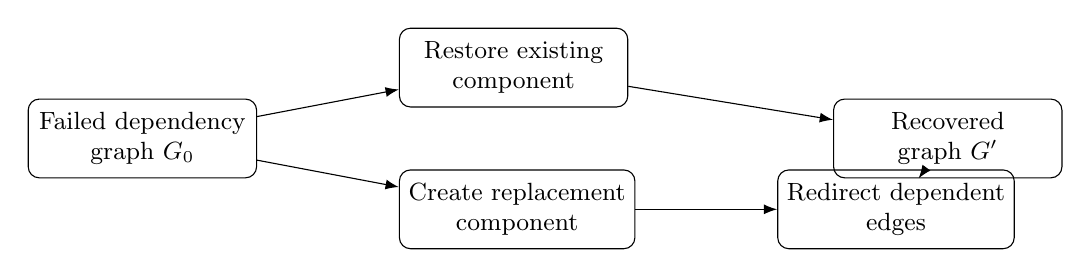
\begin{tikzpicture}[>=Latex,node distance=15mm and 18mm,box/.style={draw,rounded corners,align=center,minimum width=29mm,minimum height=10mm,font=\small}]
\node[box] (initial) {Failed dependency\\graph $G_0$};
\node[box,right=of initial,yshift=9mm] (restart) {Restore existing\\component};
\node[box,right=of initial,yshift=-9mm] (birth) {Create replacement\\component};
\node[box,right=of birth] (rewire) {Redirect dependent\\edges};
\node[box,right=26mm of restart,yshift=-9mm] (goal) {Recovered\\graph $G'$};
\draw[->] (initial) -- (restart);\draw[->] (initial) -- (birth);
\draw[->] (restart) -- (goal);\draw[->] (birth) -- (rewire);\draw[->] (rewire) -- (goal);
\end{tikzpicture}
\caption{Two recovery routes: restoration of an existing component, or creation followed by rewiring. Each arrow is a costed action; the lower route requires both operations.}\label{fig:concept}
\end{figure}

\begin{table}[H]\centering\caption{Actions in the three-service synthetic recovery instance.}\label{tab:actions}
\begin{tabularx}{\linewidth}{@{}lclX@{}}\toprule
Action & Cost & Prerequisite & State change\\\midrule
Restart authentication & 3 & None & Marks the original authentication service operational\\
Create replacement & 2 & None & Adds an operational replacement authentication service\\
Rewire reporting & 1 & Replacement created & Replaces the reporting-to-original edge with a reporting-to-replacement edge\\\bottomrule
\end{tabularx}\end{table}

\section{Exact search and verification}
We use two complementary exact procedures. Exhaustive enumeration supplies a finite audit trail for a small action set, while uniform-cost search provides an exact shortest-path baseline over the reachable state graph. Their agreement checks the model and implementation without implying that either algorithm is new.

\Cref{alg:enumeration} enumerates ordered subsets of distinct actions. Because every action occurs at most once, the number of candidate sequences before feasibility pruning is $\sum_{j=0}^{|A|}|A|!/(|A|-j)!$.
\begin{algorithm}[H]\caption{Exhaustive finite repair oracle}\label{alg:enumeration}
\begin{algorithmic}[1]
\Require Initial state $s_0$, actions $A$, budget $B$, goal predicate
\State $W\gets\varnothing$
\For{each ordered subset $\pi$ of distinct actions from $A$}
  \State Simulate $\pi$ from $s_0$ in order
  \If{all actions are applicable, constraints hold, and $\Cost(\pi)\le B$}
    \If{$\Goal(T_\pi(s_0))$} \State $W\gets W\cup\{(\Cost(\pi),\pi)\}$ \EndIf
  \EndIf
\EndFor
\State \Return the minimum-cost entries in $W$, or infeasible if $W=\varnothing$
\end{algorithmic}
\end{algorithm}

\Cref{alg:ucs} uses a priority queue and a key containing both graph state and used-action history. Omitting history would be unsound for the prerequisite rules used here.
\begin{algorithm}[H]\caption{Uniform-cost repair search}\label{alg:ucs}
\begin{algorithmic}[1]
\Require Initial state $s_0$, finite actions $A$, nonnegative costs
\State $d[s_0]\gets 0$; initialize priority queue $Q\gets\{(0,s_0)\}$
\While{$Q\ne\varnothing$}
  \State Remove minimum-cost pair $(g,s)$ from $Q$
  \If{$g\ne d[s]$} \State \textbf{continue} \EndIf
  \If{$\Goal(s)$} \State \Return $g$ \EndIf
  \For{each applicable unused action $a$}
    \State $s'\gets T_a(s)$; $g'\gets g+c(a)$
    \If{$s'$ is permitted and $g'<d.get(s',+\infty)$}
      \State $d[s']\gets g'$; insert $(g',s')$ into $Q$
    \EndIf
  \EndFor
\EndWhile
\State \Return infeasible
\end{algorithmic}
\end{algorithm}

\begin{proposition}\label{prop:ucs}
For a finite transition system with nonnegative action costs and a state key that preserves all future applicability, transition costs, and goal outcomes, \Cref{alg:ucs} returns the minimum goal-reaching cost whenever one exists.
\end{proposition}
\begin{proof}
The transition system is a finite directed graph with nonnegative edge weights. Uniform-cost search is Dijkstra's shortest-path algorithm on that graph. Its relaxation invariant ensures that a goal state removed from the queue at its current best distance cannot be improved by an undiscovered path of smaller cost. Recording history in the key prevents the identification of states with different future action sets.
\end{proof}

\section{The recovery fixture}
The initial graph contains an operational ingress service, a failed authentication service, and an operational reporting service. Reporting depends on authentication and is therefore unusable until that dependency is repaired. The two successful minimum-cost paths are shown in \Cref{fig:fixture} and listed in \Cref{tab:fixture}.
\begin{figure}[H]\centering
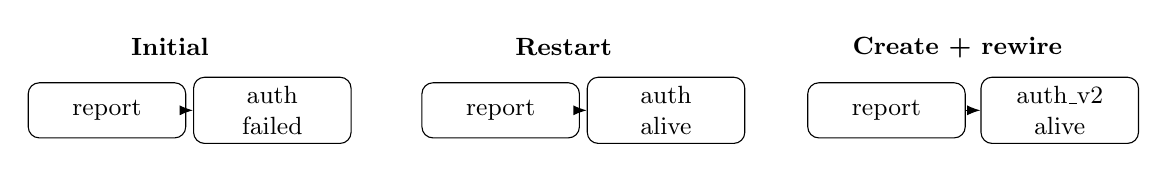
\begin{tikzpicture}[>=Latex,svc/.style={draw,rounded corners,minimum width=20mm,minimum height=7mm,font=\small},every node/.style={align=center}]
\node[font=\bfseries\small] at (0,1.15) {Initial};
\node[svc] (r0) at (-.8,.35) {report};\node[svc] (a0) at (1.3,.35) {auth\\failed};\draw[->] (r0)--(a0);
\node[font=\bfseries\small] at (5,1.15) {Restart};
\node[svc] (r1) at (4.2,.35) {report};\node[svc] (a1) at (6.3,.35) {auth\\alive};\draw[->] (r1)--(a1);
\node[font=\bfseries\small] at (10,1.15) {Create + rewire};
\node[svc] (r2) at (9.1,.35) {report};\node[svc] (a2) at (11.3,.35) {auth\_v2\\alive};\draw[->] (r2)--(a2);
\end{tikzpicture}
\caption{Dependency edge before recovery and after the two alternative optimal repairs. The ingress component, unchanged in all three configurations, is omitted for clarity.}\label{fig:fixture}
\end{figure}

\begin{table}[H]\centering\caption{Exact recovery results for the three-service fixture.}\label{tab:fixture}
\begin{tabularx}{\linewidth}{@{}Xccc@{}}\toprule
Action sequence & Total cost & Goal reached? & Optimal?\\\midrule
Restart authentication & 3 & Yes & Yes\\
Create replacement; rewire reporting & 3 & Yes & Yes\\
Create replacement only & 2 & No & No\\
No action & 0 & No & No\\\bottomrule
\end{tabularx}
\end{table}

An exhaustive certificate enumerates all $1+3+6+6=16$ ordered subsets of the three actions. Exactly four sequences pass the fixture's applicability and budget checks; two reach the goal, both at cost three. The independent exact procedures agree on this optimum. This is a correctness test for the encoded rules, not evidence that creation always reduces repair cost.

\section{Synthetic scaling study}
To test search behavior beyond one example, we construct a family of $n$ independent failed-service groups. Each group offers a restart of cost three, or creation of cost two followed by rewiring of cost one. The global goal requires recovery of every group. Three deterministic action-order seeds are used for each $n\in\{1,2,3,4\}$, giving 12 executions over four underlying graph sizes. These seeds change action ordering, not graph topology or repair costs. Both exact methods must return $3n$. The experimental design is summarized in \Cref{tab:design}.
\begin{table}[H]\centering\caption{Experimental design and checks for the synthetic search comparison.}\label{tab:design}
\begin{tabularx}{\linewidth}{@{}lX@{}}\toprule
Property & Setting\\\midrule
Repair groups & $n=1,2,3,4$\\
Actions per group & Three: restart, create, rewire\\
Action-order seeds & $0,1,2$ for each $n$\\
Total instances & 12\\
Methods & Exhaustive enumeration and uniform-cost search\\
Correctness check & Exact agreement on minimum cost $3n$\\
Reported search metric & Nodes visited by exhaustive enumeration; states expanded by uniform-cost search\\
Scope & Synthetic independent groups; no matched GROOVE experiment\\\bottomrule
\end{tabularx}\end{table}

The results in \Cref{tab:scaling} show that uniform-cost search explores substantially fewer nodes than enumeration in the reported cases. The methods do not measure precisely identical quantities: enumeration counts visits in its search tree, including repeated configurations, while uniform-cost search counts settled state expansions. The difference is meaningful for the implemented algorithms but must not be interpreted as an advantage over GROOVE or as a novel reduction result.
\begin{table}[H]\centering\caption{Selected deterministic search counts from the successful automated experiment. Each listed count is reproduced across the three action-order seeds.}\label{tab:scaling}
\begin{tabular}{@{}rrrrr@{}}\toprule
Groups $n$ & Actions & Optimal cost & Enumeration visits & UCS expansions\\\midrule
3 & 9 & 9 & 3,796 & 78\\
4 & 12 & 12 & 314,217 & 399\\\bottomrule
\end{tabular}
\end{table}

\Cref{fig:scaling} plots these counts on a logarithmic axis to retain both series on a readable scale. No inference about asymptotic complexity is drawn from two displayed sizes.
\begin{figure}[H]\centering
\begin{tikzpicture}[x=1.3cm,y=.65cm]
\draw[->] (0,0)--(5.8,0) node[right]{Groups};\draw[->] (0,0)--(0,9.2) node[above]{${\log}_{10}(\mathrm{count})$};
\foreach \y/\lab in {0/0,3/2,6/4,9/6}{\draw (-.07,\y)--(.07,\y) node[left=3pt]{\small\lab};}
\foreach \x/\lab in {2/3,4/4}{\node[below] at (\x,0) {\small\lab};}
% vertical scale is 1.5 drawing units per log10 unit
\draw[very thick] (2,5.369)--(4,8.246);
\draw[very thick,dashed] (2,2.838)--(4,3.901);
\fill (2,5.369) circle (2pt);\fill (4,8.246) circle (2pt);
\fill (2,2.838) circle (2pt);\fill (4,3.901) circle (2pt);
\node[anchor=west,font=\small] at (4.1,8.25) {Enumeration};
\node[anchor=west,font=\small] at (4.1,3.9) {UCS};
\end{tikzpicture}
\caption{Search effort for three and four independent repair groups on a logarithmic plotting scale. Points represent counts from \Cref{tab:scaling}, not runtime or memory.}\label{fig:scaling}
\end{figure}

\section{Exact decomposition and its boundary}
The synthetic family admits an additional analysis. If local actions cannot influence other groups, the global optimization problem separates. The decomposition is mathematically elementary, but its conditions provide a useful check against unjustified reduction.
\begin{proposition}\label{prop:decomp}
Suppose the global state is the product of $n$ local states; each action changes exactly one local state, with applicability and cost depending only on that local state; the goal is the conjunction of local goals; and no cross-group safety or resource restriction applies. Then
\begin{equation}\label{eq:decomp}\Opt(s_0)=\sum_{i=1}^{n}\Opt_i(s_{0,i}).\end{equation}
Moreover, concatenating one optimal plan for each local problem produces a globally optimal plan. The evaluated implementation reports only the optimum cost, not the concatenated plan.
\end{proposition}
\begin{proof}
Project any feasible global plan onto the actions of group $i$. Locality ensures that each projection is a feasible plan for that group's goal. By additivity, the global plan costs at least the sum of local optima. Conversely, concatenate optimal local plans. Their actions commute with those of other groups in the sense of preserving applicability and outcomes, so the concatenation reaches every local goal and attains the lower bound.
\end{proof}

\Cref{alg:decomp} implements the guarded decomposition. The guard is part of the method: a cost identity derived under independence cannot be used without checking independence. In the evaluated code, declared coupling edges or a global resource limit trigger rejection; this is not a general automated proof of semantic independence. The sufficient syntactic certificate developed below explains what a broader implementation would have to check.
\begin{algorithm}[H]\caption{Guarded component-wise exact repair}\label{alg:decomp}
\begin{algorithmic}[1]
\Require Repair instance $I$, proposed partition $\{I_1,\ldots,I_n\}$
\If{an action, goal, constraint, or resource couples different groups}
  \State \Return ``decomposition not certified''
\EndIf
\For{$i\gets1$ to $n$}
  \State $c_i\gets\Call{UniformCostRepairCost}{I_i}$
\EndFor
\State \Return $\sum_i c_i$
\end{algorithmic}
\end{algorithm}

\subsection{A sufficient syntactic independence certificate}
For a finite, explicitly factored state description, let $X=\dot\bigcup_{i=1}^n X_i$ be disjoint sets of state variables. For every action $a$, let $R(a)$ and $W(a)$ denote conservative read and write footprints, including every variable used by its precondition, effect, or action-dependent cost. A partition is \emph{syntactically certified} if each action belongs to exactly one group $i$ with $R(a)\cup W(a)\subseteq X_i$, every goal predicate factors as $\bigwedge_i\Phi_i(X_i)$, and every admissibility or resource predicate factors into local predicates. Any unclassified global resource, cross-component edge, or uncertain footprint causes rejection.
\begin{proposition}[Soundness of a local-footprint certificate]\label{prop:footprint}
For a finite transition system with complete conservative action footprints, local costs, a product initial state, and factorized goals and admissibility, acceptance of the syntactic certificate implies the hypotheses of \Cref{prop:decomp}. Consequently the sum of local optimum costs is the global optimum whenever each local problem is feasible.
\end{proposition}
\begin{proof}
Because the read and write footprints of every action are contained in one variable block, executing it cannot change another block or depend on another block's value. Complete footprints include all cost and applicability dependencies. Factorized admissibility and goals prohibit hidden cross-block restrictions. Thus every feasible global action sequence projects to feasible local sequences, and any concatenation of feasible local sequences remains admissible. The two inequalities in the proof of \Cref{prop:decomp} therefore apply.
\end{proof}
The certificate is conservative: rejection does not imply that decomposition is impossible. The certificate and \Cref{prop:footprint} are an analytical sufficient condition, \emph{not} a claim that the published experimental code extracts read/write sets or implements a general-purpose static analyzer. Shared restart capacity violates factorization and is correctly outside the certificate's scope.

Twenty-four synthetic decomposition executions were completed, using $n=1,\ldots,8$ and three action-order seeds; the seeds do not generate independent dependency topologies. Every case returned the expected total cost $3n$; for $n\le4$, full-state uniform-cost search independently agreed. \Cref{tab:decomp} distinguishes these checks from the unperformed large-instance full-state comparisons.
\begin{table}[H]\centering\caption{Scope of the decomposition validation.}\label{tab:decomp}
\begin{tabularx}{\linewidth}{@{}p{0.25\linewidth}X X@{}}\toprule
Groups & Decomposition check & Independent full-state check\\\midrule
$1$--$4$ (12 cases) & Cost $3n$ in all cases & UCS agreement in all cases\\
$5$--$8$ (12 cases) & Cost $3n$ in all cases & Not performed\\
Two coupled groups & Coupling guard rejects partition & Independent restart--restart plan violates shared capacity\\\bottomrule
\end{tabularx}\end{table}

The coupling counterexample is concrete. Consider two groups with a shared capacity permitting at most one restart. Independent local optimization can choose a restart for each group, producing a cost-six plan that is infeasible under the shared constraint. Alternative creation-and-rewiring choices can retain the same numerical optimum in this example; equality of objective values does not certify the validity of the returned plan. The distinction between preserving cost and preserving solutions is illustrated in \Cref{fig:coupling}.
\begin{figure}[H]\centering
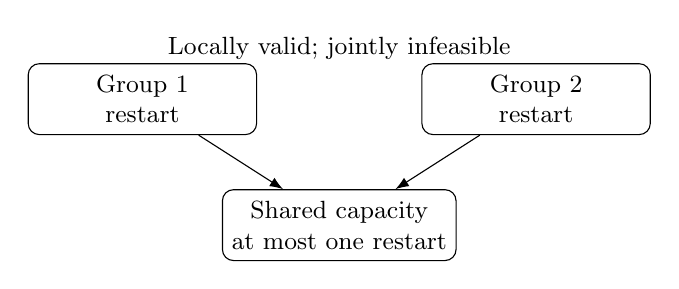
\begin{tikzpicture}[>=Latex,box/.style={draw,rounded corners,align=center,minimum width=29mm,minimum height=9mm,font=\small}]
\node[box] (a) at (0,0) {Group 1\\restart};\node[box] (b) at (5,0) {Group 2\\restart};
\node[box] (cap) at (2.5,-1.6) {Shared capacity\\at most one restart};
\draw[->] (a)--(cap);\draw[->] (b)--(cap);
\node[font=\small] at (2.5,.65) {Locally valid; jointly infeasible};
\end{tikzpicture}
\caption{A shared restart limit breaks the noninterference assumption. A partition guard must reject the naive concatenation of locally chosen repair plans.}\label{fig:coupling}
\end{figure}


\section{Fresh identities, equivariance, and exact quotient search}
A replacement identity is operationally relevant when a dependency points to it, but its arbitrary spelling need not be relevant. Let $I_0$ be the finite set of identities present initially, and let $F$ be a bounded set of fresh identities. A permutation $\sigma$ of $F$ fixes $I_0$ and acts simultaneously on vertex names, edge endpoints, attributes containing identities, and history-relevant facts. Write $\sigma s$ for the resulting state. Two states are \emph{fresh-name equivalent}, $s\sim_N t$, if $t=\sigma s$ for such a permutation. Only well-typed permutations preserving service roles are permitted.

A transition system is \emph{equivariant} if each admissible transition $s\xrightarrow{a,w}t$ has a corresponding transition $\sigma s\xrightarrow{\sigma a,w}\sigma t$ and conversely, where $w$ is the action cost. Its goal predicate and safety constraints must be invariant under these permutations. In particular, negative application conditions, capacity reservations, and allocation policies must be preserved. Name-dependent prices, hard-coded identity tests, or global fresh-name counters can invalidate the hypothesis. History is renamed along with the graph, rather than discarded.

\begin{proposition}[Fresh-name quotient preserves optimal recovery]\label{prop:symmetry}
For a finite, nonnegative-cost, equivariant repair transition system with permutation-invariant goals and admissibility, the orbit quotient $\mathcal S/{\sim_N}$ preserves goal reachability and the minimum goal-reaching cost from every initial state. A quotient path can be lifted to a concrete path with the same cost.
\end{proposition}
\begin{proof}
Each transition $s\xrightarrow{a,w}t$ induces an orbit transition $[s]\xrightarrow{w}[t]$. This is well defined: for any other representative $s'=\sigma s$, equivariance supplies $s'\xrightarrow{\sigma a,w}\sigma t$, whose target is in $[t]$. Conversely, an orbit transition from $[s]$ may be represented by a transition starting at an arbitrary chosen representative of $[s]$ by applying the inverse renaming. Repeating this lifting step constructs a concrete path for every quotient path, with the same sequence of weights. Projection of concrete paths gives quotient paths with unchanged weights. Goal and admissibility invariance ensure that projection and lifting preserve feasibility and success. The sets of attainable goal-reaching path costs therefore coincide, so their minima coincide.\end{proof}

The proposition is an application of established symmetry and nominal reasoning, not a claim that quotient-state optimality was first discovered here \cite{Fernandez2005,Burch1992,Emerson2005,Konig2025}. Its value for the repair model is to specify exactly which identity-bearing facts must survive renaming. A coarse count of live vertices, edges, and creations is not an adequate substitute for an orbit key: counts can agree even when the dependency structure and future reachability differ.

\begin{algorithm}[H]\caption{Exact search over certified fresh-name orbits}\label{alg:orbit}
\begin{algorithmic}[1]
\Require Finite equivariant repair system, initial state $s_0$, canonical orbit key $K$
\State $d[K(s_0)]\gets0$; $Q\gets\{(0,s_0)\}$
\While{$Q\ne\varnothing$}
  \State Remove minimum-cost pair $(g,s)$ from $Q$
  \If{$g\ne d[K(s)]$} \State \textbf{continue} \EndIf
  \If{$\Goal(s)$} \State \Return $g$ \EndIf
  \For{each admissible successor $s'$ of $s$ with cost $w$}
    \If{$g+w<d.get(K(s'),+\infty)$}
      \State $d[K(s')]\gets g+w$; insert $(g+w,s')$ into $Q$
    \EndIf
  \EndFor
\EndWhile
\State \Return infeasible
\end{algorithmic}
\end{algorithm}

\Cref{alg:orbit} is correct under the hypotheses of \Cref{prop:symmetry}, provided $K(s)=K(t)$ exactly for states in the same permitted orbit. Computing a canonical key may itself be expensive, and the algorithm is presented as a mathematically justified design, not as a benchmarked improvement. The public repair benchmark currently evaluates ordinary uniform-cost search, not orbit-quotient search.

\begin{table}[H]\centering\caption{Fresh-name equivalence conditions and failure modes.}\label{tab:symmetry}\small
\begin{tabularx}{\linewidth}{@{}p{0.35\linewidth}X@{}}\toprule
Condition & Consequence for quotient search\\\midrule
Roles, dependency endpoints, and history renamed consistently & Structural and rule-relevant information is retained\\
Costs, goals, and constraints invariant under permitted permutations & Equal-cost transitions and goal outcomes are preserved\\
Name-dependent action cost or identity-specific prohibition & Renaming is not generally sound; the partition must be rejected\\
Global capacity or negative condition referencing identities & Must be explicitly checked for equivariance; cannot be ignored\\\bottomrule
\end{tabularx}\end{table}

A small executable regression accompanies the manuscript. It tests two permutations of interchangeable replacement labels, each with creation cost two and rewiring cost one, and confirms an optimum of three. It also checks a deliberately identity-dependent cost rule that violates equivariance. These are \emph{unit tests of the assumptions}, not a measured state-space reduction or a realistic service benchmark. \Cref{tab:symmetry} summarizes the boundary; no runtime or memory improvement is inferred from the regression.

\section{Discussion and limitations}
The formal model and experiments support three restrained conclusions. First, component creation must be followed by the appropriate relationship changes when the recovery predicate depends on those relationships. Second, independent exact procedures can audit small repair spaces and reveal the cost of alternate repair sequences. Third, structural independence can make cost optimization separable, but the proof fails when a shared constraint changes global feasibility.

Several limitations are decisive. The test instances are synthetic, and the scaling family is deliberately independent. The present search comparison uses standard uniform-cost search, not a new natality-aware reduction. The state representation does not yet address concurrent actions, stochastic failures, partial observability, or real repair logs. In particular, the existing GROOVE executable check does not constitute a matched experiment on this repair model. Related work on graph transformation, model checking, abstraction, and rewriting makes this distinction essential \cite{Ghamarian2012,Emerson2005,Konig2025,Campbell2021,Adam2026,Ghasemi2026}.

The fresh-name quotient result specifies a sound abstraction under explicit equivariance assumptions, but its relationship to existing symmetry-reduction algorithms is not a novelty claim. The accompanying regression is a small illustrative check rather than a comparison of full and quotient search. The sufficient footprint certificate is a formal criterion rather than a measured algorithmic improvement; its usefulness and its relation to established independence analyses require further study. A more demanding evaluation would encode the same action costs, graph states, forbidden configurations, and recovery goals in an independently executable graph-transformation grammar. Coupled dependency networks, realistic failure traces, and comparisons against reduction methods would then be necessary to assess whether any natality-specific representation offers a benefit beyond established techniques. The present results should not be read as such a comparison. In particular, \Cref{prop:monotone,prop:essential} clarify what creation permits in an expanded action space; neither proposition establishes that graph-transformation tools cannot encode the same behavior.

\section{Conclusion}
Creation-enabled recovery can be described as an operationally directed state space with explicit identity, admissibility, and path cost. Cost-optimal repair in evolving dependency graphs is naturally expressed as a search over structural changes rather than isolated component fixes. By distinguishing restoration from replacement creation and rewiring, the formulation makes explicit why a newly created component need not immediately restore a dependent service. Exact enumeration and uniform-cost search agree on the minimum cost of a small recovery fixture and on 12 synthetic scaling instances. Under stated noninterference assumptions, the minimum cost of independent repair groups decomposes additively; 24 generated cases validate this implementation, while a shared-capacity counterexample shows why local plan choices cannot always be composed. A conservative local-footprint condition gives a sound way to certify the separability assumptions, but its general implementation and comparative evaluation remain open. Fresh-name equivariance additionally gives a sufficient condition for exact identity-quotient search, with explicit failure cases for identity-sensitive costs and constraints. These findings provide an auditable foundation for further investigation, not evidence of a novel reduction or a matched advantage over existing graph-transformation systems. Establishing those claims will require coupled workloads, independent tool-level comparison, and stronger formal results.

\section*{Data and code availability}
\begingroup\sloppy
The original implementation, synthetic fixtures, independent verification programs, and workflow-produced evidence are publicly available at \url{https://github.com/Arithmetic-Power-Geometry/The-Geometry-of-Natality}. The reproducibility record includes the successful GitHub Actions run \url{https://github.com/Arithmetic-Power-Geometry/The-Geometry-of-Natality/actions/runs/39151100642}. The additional finite symmetry-regression script is included with the present manuscript package and is not claimed to have been run by the cited repository workflow. The results reported here were generated from synthetic data; no external service logs or real-world datasets were used.

\endgroup
\section*{Declarations}
\noindent\textbf{Funding:} No external funding is reported for this study.\\
\textbf{Competing interests:} No competing interests are declared.\\
\textbf{Data provenance:} All evaluated instances are synthetic.


\section{Post-freeze independent research gates: evidence and negative findings}
\label{sec:postfreeze}
The following results were developed after the source manuscript was frozen. They do not retroactively validate any stronger claim in the original experiments.

\subsection{Conservative symmetry and decomposition gates}
Exact orbit canonicalization was implemented for a closed finite grammar, with independent finite permutation oracles. Identity-specific costs and opaque conditions remain explicit refusal cases. The certified independent-component decomposition was tested against a coupled shared-restart-capacity counterexample, where the uncoupled optimum is two and the coupled optimum is four. The standard largest-positive-savings formula for a cardinality constraint was checked on 80,973 bounded parameter cells. None of these results is claimed as a new mathematical principle.

\subsection{Frozen benchmark and performance limitations}
The frozen synthetic benchmark has 72 instances, including 36 matched and 36 negative/refusal cells. An isolated rerun measured 1,440 paired trials, with no censored outcomes. The median of nine instance-level paired wall-time differences for plain minus quotient UCS was $-3.851$ milliseconds, indicating that quotienting was slower on the tested small symmetry instances. Decomposition comparisons produced positive but very small descriptive medians; these repeated trials do not establish performance on unobserved systems. The experimental resource limit was a 60-second subprocess timeout and a two-gibibyte virtual address-space cap, not a measured two-gibibyte peak RSS.

\subsection{Creation-relay set cover and static dependency encoding}
In a closed root-to-terminal relay-creation grammar, a selected set of created relays reaches all terminals precisely when its coverage sets form a set cover. The optimization problem is therefore weighted Set Cover; this is an established reduction, not a new complexity theorem. The restricted static dependency grammar additionally supports acyclic prerequisites, a shared relay-count capacity and forbidden pairs. An independent SciPy/HiGHS mixed-integer optimizer and graph enumeration agreed on 4,096 bounded models. This external MILP solver is not a GROOVE graph-transformation baseline.

\subsection{Dynamic graph rewriting and action-time exclusions}
The bounded dynamic grammar tracks live relay names, a permanently used-name set, and directed links. Create, add-link, remove-link and delete actions are evaluated under live capacity and action-time forbidden-edge conditions. The native uniform-cost implementation and an independently enumerated NetworkX state graph agreed on 320 parameter cells, including infeasible cases. The state graph is generated independently of the native action generator, but NetworkX itself is an external shortest-path library, not an independently authored GROOVE rule interpreter.

\begin{proposition}[History-sensitive deletion defeats universal plan pruning]
\label{prop:historycounterexample}
There exists a finite nonnegative-cost creation/deletion repair instance whose only successful plans contain a deletion action, although the corresponding positive terminal-reachability grammar admits a delete-free optimum.
\end{proposition}
\begin{proof}
Take one initially unused relay identity $0$ and the goal that identity $0$ has been allocated but is no longer live. Initially $A=H=\varnothing$. Creating $0$ gives $A=H=\{0\}$; deleting it gives $A=\varnothing$ and $H=\{0\}$, satisfying the goal. Every delete-free sequence either never allocates $0$ (so $H=\varnothing$) or leaves it live (so $A=\{0\}$). Thus no delete-free plan reaches the goal. This does not contradict the restricted monotone terminal-reachability pruning argument, which excludes historical goals.
\end{proof}

\subsection{Independent originality and external semantics gate}
Existing graph transformation, set-cover, Steiner connectivity, symmetry reduction, and Dijkstra search literature prevents priority claims based solely on reformulation. The original root bibliography has 23 records, but publisher-by-publisher verification of all entries remains incomplete. The official GROOVE Generator smoke test executes a sample grammar only; no semantically matched GROOVE repair grammar with action costs, allocation history and action-time guards has been successfully executed. The present manuscript therefore remains a research-stage, full-length reconstruction rather than a submission-cleared original theorem paper.

\section{Reproducibility and audit trail}
The reproducible implementation and claim/evidence reports are retained at \url{https://github.com/Arithmetic-Power-Geometry/The-Geometry-of-Natality} on branch \texttt{research/gon-stage1-20261019}. CI evidence is recorded in Prompt 1--15 reports. All evaluated networks are synthetic. Source-to-result comparability, external validity, originality and complete reference verification remain independent publication gates.

\printbibliography
\end{document}